\date{\today}


\documentclass[11pt]{article}
\usepackage{graphicx}
\usepackage{asp2010}
\resetcounters
\bibliographystyle{asp2010}

\markboth{TAPVizieR: a new way to acess the VizieR database}{Gilles Landais, and Fran\c cois Ochsenbein}
\def\pLOcomment#1{{\bf\em #1}}

\resetcounters



\begin{document}
\title{TAPVizieR: a new way to acess the VizieR database}
\author{
        Gilles Landais, Fran\c cois Ochsenbein, Anne-Camille Simon
\affil{Centre de Donn\'ees astronomiques de Strasbourg (CDS) }}

\begin{abstract}
VizieR is a component of the Virtual Observatory: it provides tables of
catalogs to external softwares with VO standards like the VOTable output.
Accessing VizieR with the ADQL/TAP standard represents a new milestone
in the VizieR access facilities.
%Due to the heterogeneity and huge volumetry of the VizieR contents, 
%the TAP implementation required a few adaptations.

The PostgreSQL engine has been chosen to store data: it provides a solid
database containing utilities to manage SQL or to create the customized
HEALPix indexing ``H3C'' which permits a fast access from sky coordinates.
The TAP standard however was not designed to accomodate databases
managing tens of thousands of tables like VizieR, and some compromises
with the TAP standard were necessary in this first version of TAPVizieR.
\end{abstract}

%------------------------------------------------------------------------------
% INTRODUCTION
%------------------------------------------------------------------------------


%------------------------------------------------------------------------------
%
\section{The context}
%VizieR \citep{F.Ochsenbein, 2000A&AS..143...23O} is a component of the Virtual 
%Observatory, it provides tables of catalogs to external softwares with VO 
%standards like the VOTable output format.
%A new milestone consists in the integration of the ADQL/TAP standards in VizieR.

ADQL \citep{adql_2011} is an other way to query VizieR tables 
\citep{ochsenbein_2000}; ADQL is an extension of SQL 
%extension adapted for astronomy with adding 
with additional astronomical functions and geometrical objects. 
It enables the usage of formulae involving column combinations which can be used 
for display or to filter a set of records (\textit{see fig.\ref{P044:ADQLexample}}). 
%
That kind of operations were limited in the VizieR application and required 
the usage of external softwares for such computations.

\begin{figure}[!h] \center
\begin{footnotesize}%\begin{scriptsize}
\begin{verbatim}
SELECT ra_icrs_, de_icrs_, BTmag-VTmag as B-V
FROM   tyc2
WHERE  1=CONTAINS(POINT('ICRS', ra_icrs_, de_icrs_),
                  CIRCLE('ICRS', 244.26, -22.98, 10/60.))
   AND BTmag-VTmag<1
\end{verbatim}\end{footnotesize}%\end{scriptsize}
\caption{Example of an ADQL query on the catalog Tycho using a color 
constraint (BTmag-VTmag) and a cone search arround M80.}\label{P044:ADQLexample}
\end{figure}

TAP \citep{tap_2011} is a protocol to execute an ADQL query 
on a remote database. 
TAP services are already available in data centers like CADC or GAVO, and
some external software like TOPCat or TAPHandle can work with
the standard. These applications link tables coming from different databases
(GAVO, CADC and now VizieR) with a unique interface and use the same language.
They offer real extended possibilities for astronomers who can combine 
tables stored in different places. %data center.


%------------------------------------------------------------------------------
% DEDICATED DATABASE
%------------------------------------------------------------------------------
\section{A dedicated database}

\subsection{Homogenize the storage}
The VizieR application provides catalogs. The tables and their metadata (descriptions) 
are stored in a transactionnal database, or in dedicated binary files
for the large catalogs (e.g. WISE, 2MASS, SDSS, etc.) in order to speed up the 
search by position.

%There are different kinds of storages used in VizieR. The common tables are 
%stored in a transactionnal database Sybase or PostgreSQL. The large tables are 
%stored in binary files in order to speed up the search by position; these tables
%concerns the large suveys like 2MASS, SDSS, WISE, etc.

ADQL based on SQL requires %assumes to work with 
transactionnal database or %some
technologies like Hadoop. We think that SQL is the more practical way
to be ADQL-compatible, so, we chose to create a new dedicated database which
gathers all catalogs. 

This new database is a PostgreSQL engine which supports effectively 3.5 Tb
of data and indexes.
With PostgreSQL, we gain the replication capabilities and some easy way
to create advanced functions.

\subsection{Indexation}
VizieR has tables that can contain up to 1 billion records. This volumetry
needs indexation and in particular a positionnal indexation, because conesearch
or crossmatch (join tables according to their positions) are the most popular 
functionalities in VizieR.

In PostgreSQL an index by position can be built with libraries like {\em PgSphere}
provided by PostgreSQL; an external plugin {\em Q3C}
was also developed 
by \citet{q3c_2006} for astronomical applications.
The PgSphere is user-friendly; however, Q3C minimizes resources and
is more efficient with tables containing over one million of records --- %\\
therefore better suited for VizieR.
%It is obvious than Q3C is a better way for VizieR!
Q3C works with the quadcube algorithm; % and provides a set of functions. 
however, {\em HEALPix} is more and more becoming a standard in
%more and more the HEALPix standard is used by applications 
astronomical applications like 
%(\textit{ex.:} 
Aladin, the CDS Crossmatch service, GAIA, etc.
%So, to improve the interoperability between services, it would be better to use a HEALPix index.

%However, the Q3C index and his functions works with the Qbox algorithm and we 
%thought that HEALPix would be a better way to link external applications which
%work with it (\textit{ex.:} Aladin, the CDS Crossmatch service, GAIA, etc.).\\

\paragraph{The H3C library}

We built a 2D PostgreSQL library \textbf{H3C} 
(\textit{i.e. \textbf{H}ealpiX-\textbf{T}ree-C code}), largely inspired from
 Q3C, with the same functionalities --- with the exception that
the functions dealing with polygons are available 
for convexes only.

The tessellation of the sphere with HEALPix cells requires however
a deep resolution 
to be as efficient as Q3C. This implementation was possible thanks to the recent
improvement of the  HEALPix 64bits C++ library maintained by the Nasa 
\citep{gorski_healpix}.

%H3C uses the C++ library provided by the nasa 
%\citep{Gorski, 2011ascl.soft07018G} who improved the library facilities to work
%with 64-bit integers. 64-bit integers are required if we want to compare the 
%Q3C efficiency with H3C: we have to work, indeed, with a good precision 
%(\textit{nside=15}). Thank to the nasa which improve for our usage the library!

\paragraph{Some comparisons between libraries} (\textit{see fig.\ref{P044:comparative}})
About efficiency, the tests show than Q3C and H3C are largely better than 
PgSphere. Moreover the size required by the index
as well as the time required for their creation
are significantly smaller with Q3C/H3C than with PgSphere.

\begin{figure}[htp] \center
\begin{small}
\begin{tabular}{lllll}% \hline
 & PgSphere & Q3C & H3C & H3C  \\
 &          &     &     &{\scriptsize cluster index} \\ %\hline
conesearch in 2mass (M1, radius:2arcsec) & 340ms& 360ms& 380ms &\\ %\hline
conesearch in 2mass (M1, radius:2arcmin) & 500ms& 390ms& 400ms &\\ %\hline
conesearch in 2mass (M1, radius:2deg)    & 88s& 4.3s& 1.26s &\\ %\hline
crossmatch Tycho-hipparcos & 110s & 4.5s &  4.5s & 3s\\ %\hline
crossmatch 2mass-hipparcos & 48min & 15min & 14min & 6.5min\\ %\hline
crossmatch 2mass-Tycho     & 4h30 & 49min  & 48min & 11.5min\\ %\hline
\end{tabular}
\end{small}
\caption{Comparisons of the positional indexation applied to Hipparcos 
($\sim$100K records), Tycho ($\sim$2.5M records) and 2mass ($\sim$450M records)
catalogues. All tests are performed on the same Linux computer (99G RAM) using a
PostgreSQL (version 9.1) database. The cache disk was deleted before each test.}
\label{P044:comparative}
\end{figure}

\paragraph{Managing the coordinate systems}

The coordinate system used in VizieR tables depend on the catalog, but VizieR 
can compute positions of any catalog in another coordinate system than the 
original one, taking into account the proper motions when these are 
described in the VizieR METAdata.

Working with a unique coordinate system is obviously more efficient
in ADQL, especially for crossmatches. So, we are adding the position in 
the ICRS frame in each table; 
the new columns (\_ra.icrs, \_de.icrs) are computed for the epoch J2000 
if proper motions are known.

%ADQL contains geometrical objects defined by a region in a given coordinate 
%system. However, the ADQL list of coordinate systems is restricted 
%(\textit{e.g.: ICRS, FK4, ...}) and is not sufficient to deal with all 
%tables in VizieR (because equinox/epoch can be different than the
%main coordinate system used in ADQL).
%
%Moreover, VizieR can compute positions of every catalog in an other coordinate
%system than the original, taking into account the known proper motions.
%
%Working in a unique coordinate system is obviously better in the ADQL context
%in which we can more easily join tables according to their positions. 
%So, we are homogenizing coordinate systems by adding position in ICRS
%for each tables. This re-ingestion of tables creates new columns
%(\_ra.icrs,\_de.icrs), computed at the epoch J2000 if proper motions are known.


%------------------------------------------------------------------------------
% VIZIER IMPLMENTATION
%------------------------------------------------------------------------------
\section{TAPVizieR implementation}

\subsection{Technologies and library used}
\paragraph{The database}


The TAPVizieR service uses a PostgreSQL database and takes advantage of the
C-functions to index positions using H3C;  functions dealing with 
coordinate conversions were also added on the server side.
%use the {\em as4} library made by \textit{F.Ochsenbein (CDS).}

%The TAPVizieR service uses a PostgreSQL database, it takes advantage with the 
%C-functions to index positions : H3C uses the function 
%which returns an healpix number from position in degree for indexing in a btree
%functional index. %The library H3C uses the C++ library made by the Nasaa.
%
%The TAPVizieR database contains functions to convert position in an other 
%coordinate system with using the AS4 library made by \textit{F.Ochsenbein (CDS).}

\paragraph{Parsing the ADQL query and providing data with TAP}

The TAP/ADQL service is a Web application written in Java. 
We use the UWS/TAP and ADQL libraries \citep{simbad_tap_2011}, 
helpful to translate ADQL into an object tree 
easily handled to take into account the VizieR METAdata. 

%The TAP/ADQL service is a Web application in JAVA. It uses the Java library
%made by \textit{CDS} \citep{simbad_tap_2011} for UWS/TAP and ADQL. This is a helpful
%library, in particular to translate ADQL into an object tree easily handled
%to take into account the VizieR METAdata. We adapted the library to transform
%ADQL into a SQL containing AS4-H3C functions.

\paragraph{Architecture}
The TAPVizieR architecture is composed of the TAP/ADQL web application, a VizieR
mirror and a PostgreSQL installation (\textit{see fig.\ref{P044:architecture}}).
The database is composed of a master and a standby databases using
the synchronous replication available in PostgreSQL since the version 9.1.
The pool {\em PgBouncer} is also used to manage database connections, and to
enable a precise configuration. 

\begin{figure}[hbp] \center
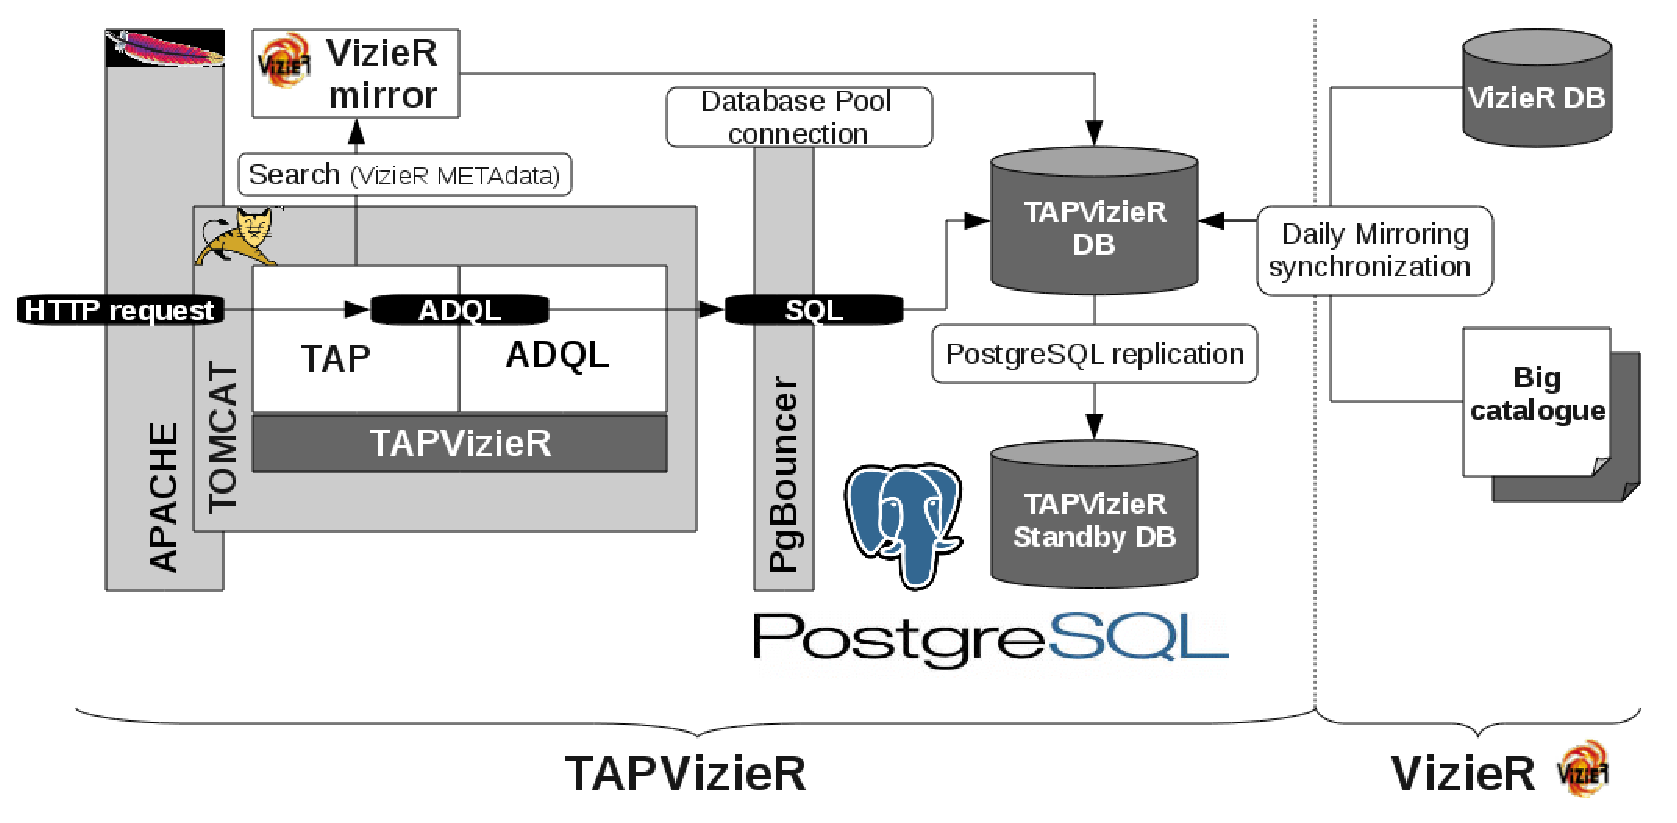
\includegraphics[width=0.85\textwidth]{P044_fig1.eps}
\caption{The TAPVizieR architecture}\label{P044:architecture}
\end{figure}

\subsection{The Web interface}
\label{P044:web_interface}
2 modes are available to query tables in TAPVizieR.
The first, the {\em TAP mode}, is
following the TAP protocol; it consists in a set of standardized URLs
which
describe and execute an ADQL Query. This mode, used by external TAP-compatible
software, is available from
{\small\url{http://tapvizier.u-strasbg.fr/TAPVizieR/tap/(tap_service_name)}}

The second mode consists in a web interface %which is an easy way to use TAPVizieR.  This web page is 
available at {\small\url{http://tapvizier.u-strasbg.fr/adql/}}, where
commonly used ADQL queries can easily be generated.

The technologies used are Ajax/JQuery/JSON to query TAPVizieR in asynchronous 
TAP mode. The web mode uses some TAP extension, like a \textit{"/search"} service
in which the rich METAdata available in VizieR are used in order to retrieve tables 
from position, keywords, authors, etc.

%In particular, a simple text search uses the service \textit{"/search?source=..."}.
%to find tables among the $\sim$20,000 VizieR tables. This URL isn't a
%TAP standard ; it is an added capability useful for astronomers.\\
%In background, the TAPVizieR application queries a VizieR mirror by HTTP: this 
%method uses VizieR METAdata, more detailed than the TAP METAdata and have 
%coverage informations which enable a search by position 
%(by name or coordinates).

%In addition to the search, the web page can generate ADQL from a simple form.
%choice of columns to display, constraints applied to columns, cone search or 
%crossmatch by position, etc.

%Finaly the ADQL query can be modified by advanced users with adding their own 
%formula.

%\begin{figure}[hbp] \center
%\includegraphics[width=0.75\textwidth]{capture-webpage.eps}
%\caption{The TAPVizieR web page}\label{P044:webpage}
%\end{figure}


\subsection{Departures from standards}

\paragraph{A big volumetry}

The VizieR database is huge:  3.5Tb constituted by 10,000 catalogues, 20,000
tables and more than 300,000 columns of tables. The TAP standard requires
to return the TAP schema as a single XML output file. Such an output represents
$\sim$86Mb, which is too huge to be processed by a remote TAP-aware
software (in 
particular for a remote web application).

So, VizieR currently returns only the table descriptions without the 
column description ($\sim$3.5Mb). 
An additional service (\textit{i.e. an other URL}) provides a full
description of a specified table; this service is not (yet) a TAP standard.

\paragraph{Understanding the coordinate system}

%The coordinate system parameter is not standard in the TAPVizieR service.
%If it is used in the SELECT part of an ADQL query the coordinate system 
%parameter is used in OUTPUT . So, you can use the possibility to make a 
%change of coordinate system.
%(example: SELECT POINT('FK4', ra\_icrs,de\_icrs\_) from tyc2)
%This syntax should evolve in the future with ADQL evolutions.
%
%Else the parameter is used in INPUT.
%If the coordinate system given differs from the actual coordinate system 
%(given by the VizieR METAdata), then the TAPVizieR service will replace the 
%parameter by the actual coordinate system. In that case, the application will 
%send Warnings.
%In the case of a crossmatch on columns in different coordinate system, 
%TAPVizieR will make a change of coordinate system (by default, it uses ICRS)

TAPVizieR makes the expected change of coordinate system in a join of 
geometrical  areas. However, the coordinate system stored in the VizieR 
METAdata is used even if the ADQL query specifies another system.

The ADQL {\em POINT} function can currently be used %in output 
to perform a change of coordinate system in the output parameters.
This syntax is not ADQL-compliant and  will evolve in the future with
the ADQL evolutions.

\section{On-going developments}

The homogenization of tables in the same coordinate system is being performed. %have to be done.
The {\em Upload} capabilities, described in TAP, will be implemented soon.
Finally, we will add a search by {\em MOC}  (Multi-Order Coverage map) 
using the HEALPix indexation \citep{O13_adassxxii}.

\bibliography{P044}
\end{document}

